% BREDEX LaTeX Template
%  \documentclass is either ``bxreport'' or ``bxarticle''
%% %                 option is bxpaper
%% \documentclass{bxarticle}
%% % ----------------------------------------------------------------------
%% \begin{document}
%% \title{}
%% \author{}
%% % \author*{Hauptautor}{Liste der Nebenautoren}
%% \maketitle
%% % ----------------------------------------------------------------------
%% \bxversion{0.1}
%% %\bxdocinfo{STATUS}{freigegeben durch}{freigegeben am}{Verteilerliste}
%% \bxdocinfo{DRAFT}{}{}{}
%% % ----------------------------------------------------------------------

%% \end{document}

\index{Add!AUT Configuration}
\index{AUT Configuration!Add}
\index{Edit!AUT Configuration}
\index{AUT Configuration!Edit}
\index{Classpath}
\index{Base Directory}
\index{Classname}
\index{CmdLineParameter}
\index{Environment}
\index{AUT!Configuration}
\index{Configuration!AUT}
\index{Activation}
\index{Application activation}
\index{AUT ID}

Once you have created a \gdproject{} \bxpref{newproject} and defined an \gdaut{} \bxpref{Defineaut}, you can add and edit \gdaut{} configurations. Use this option if you want \jb{} to start your \gdaut{} for you. 
The details in the \gdaut{} configuration tell \jb{} how to start the \gdaut{}, e.g. on which machine. 
An \gdaut{} can have multiple configurations (for example, for local and remote testing).  

\bxtipp{If you want to start your \gdaut{} yourself, and have \jb{} connect to it, then use the \bxname{gdrun} command to start the \gdaut{} \bxpref{gdrun}. In this case, you do not need to create an \gdaut{} configuration.}

The \gdaut{} configuration dialog has three different levels of detail: basic, advanced and expert. 

See the sections below for information on the different levels. 

\subsubsection{Basic \gdaut{} configuration}

You can use the basic setting (\bxfigref{autconfigbasic}) to configure your \gdaut{} if it can be started by an executable file (e.g. .bat, .exe, .cmd, .sh etc.) and if it is written in Java 1.5 or above, and you are using a Sun VM. 
\bxwarn{If you are testing RCP or GEF \gdauts{}, there are certain specific steps you need to take to configure them. See the sections on RCP testing \bxpref{rcpaut}, GEF testing \bxpref{geftest} for details. }

\begin{figure}[h]
\begin{center}
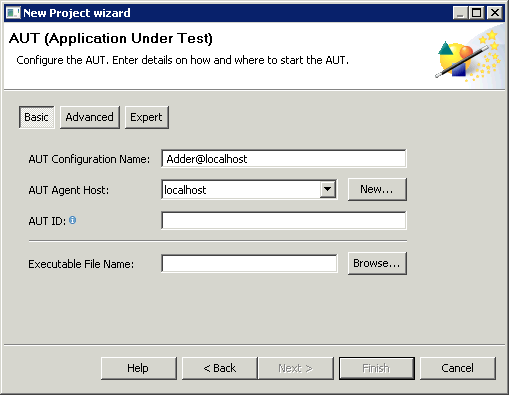
\includegraphics{Tasks/AUTs/PS/autconfigwindow_basic}
\caption{\gdaut configuration window: basic}
\label{autconfigbasic}
\end{center}
\end{figure}

\begin{enumerate}
\item A suggested name for this \gdaut{} configuration is generated automatically based on your \gdaut{} name and the default \gdserver host, specified during installation. You can change this name if you wish. 
\item The default \gdserver host is also automatically selected. You can select a new \gdserver from the combo box or add a new one by clicking \bxcaption{New}. For more information on adding and editing an \gdserver, see the  section later \bxpref{serverConfigPrefPage}.

\item Enter the executable file name in the \bxname{Executable File Name} field. This path can be relative if you define a base/working directory \bxpref{AdvancedAUTConfig}).
\item Enter the \gdaut{} ID that will be given to this \gdaut{} when it is started.  
\end{enumerate}
For information on the advanced properties for the \gdaut{} configuration, see the next section \bxpref{AdvancedAUTConfig}. 

\textbf{Configuring HTML applications}\\

HTML applications have a considerably reduced configuration dialog. The information needed to start the \gdaut{} is:
\begin{enumerate}
\item the \gdaut{} configuration name (automatically generated)
\item the \gdserver{} host
\item the \gdserver{} host\gdaut{} ID
\item the base directory
\item the URL of your application
\bxwarn{Relative paths to the URL cannot be used!}
\item the browser you want to start the \gdaut{} in
\item optionally, the browser path, to use a specific version of the browser (not available for Internet Explorer). 
%\item you can also enter a \bxname{component ID tag}. If you have used a specific tag to name components in your application, enter the tag here. \jb{} will then use this information instead of the \bxname{name} attribute in the object recognition. 
\end{enumerate}

\bxtipp{HTML applications cannot currently be started using the \bxname{gdrun} command.}

\subsubsection{Advanced \gdaut{} configuration}
\label{AdvancedAUTConfig}

You can use the advanced dialog (\bxfigref{autconfigadvanced}) if your \gdaut{} is a Java JAR which can be started with a double click, or if your application can be started using the class name and the classpaths to your \gdaut{}.  The advanced configuration dialog also lets you create a working/base directory for your \gdaut{}, and add command-line arguments needed to start the \gdaut{}. You can select a JRE executable and keyboard layout.

\begin{figure}[h]
\begin{center}
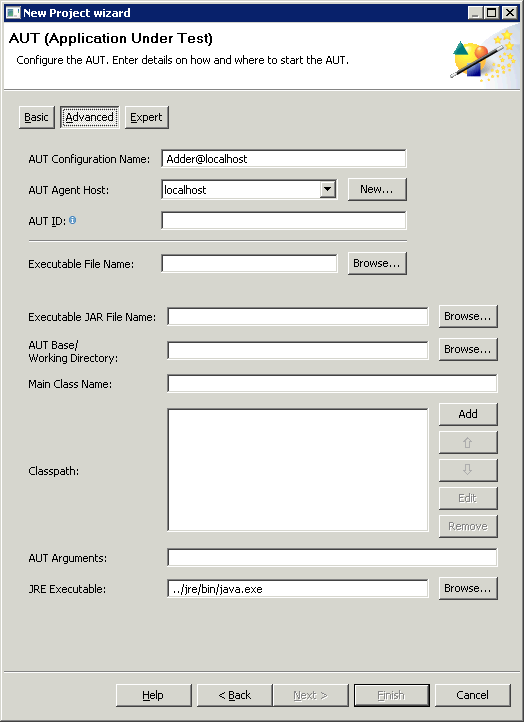
\includegraphics{Tasks/AUTs/PS/autconfigwindowadvanced}
\caption{\gdaut configuration window: advanced}
\label{autconfigadvanced}
\end{center}
\end{figure}

\begin{enumerate}
\item Enter the JAR path (directory and file
  name) into the \bxname{Executable JAR File Name} field.  

This path can be relative (if you define a base/working directory), or absolute. This JAR file must contain a manifest file which contains the main class and the classpath. 

\item You can optionally create a working/base directory to store files in. The \gdserver directory of the \jb{} installation is selected as default. To create a base directory elsewhere, browse to and select the location. 

The base directory is the working directory for any classpaths, classnames, JAR files and JRE binaries. If you create a base directory, you can enter the paths to these items using a relative path, with the base directory as the root. For more information on relative paths, read the section in the reference manual \bxextref{\jb{}efman}{ref,relativepath}. 

\item If your \gdaut{} must be started with the class name, add the main class name and the classpaths into their relative fields. The paths can be relative (if you have defined a base directory), or absolute. 
\bxtipp{Add all the necessary files and directories to start the \gdaut{}. }
\item Enter any necessary command-line arguments for the \gdaut{} in the
 \bxname{AUT Arguments} field. 
\item Browse to a JRE executable or add a new one by clicking \bxcaption{New}. 
The Java version used must be 1.4 or later. For more information on adding a new JRE executable for this \gdserver, see the later section \bxpref{serverConfigPrefPage}. 

Java is installed with \jb{}. You can find the Java file in:\\
\bxmenu{\jb{}}{jre}{bin}.
Use java.exe if you want to use a console, use javaw.exe if you do not want a console. 
\item For SWT and RCP \gdauts{}, select which keyboard layout is used on the machine on which the \gdaut{} will run. 

\bxtipp{The keyboard layout is not the actual keyboard attached to the computer, but is based on the regional language settings for the operating system.}

\jb{} supports English (US) and German (DE) keyboard layouts out-of-the box. If you want to use a different keyboard layout, see the reference manual for information on creating keyboard layouts \bxextref{\jb{}efman}{ref,keyboardlayout}. 
\end{enumerate}
For information on the expert properties for the \gdaut{} configuration, see the next section \bxpref{ExpertAUTConfig}. 

\subsubsection{Expert \gdaut{} configuration}
\label{ExpertAUTConfig}
You can use the expert dialog (\bxfigref{autconfigexpert}) to configure more detailed information about how the \gdaut{} should be started. 

\begin{figure}[h]
\begin{center}
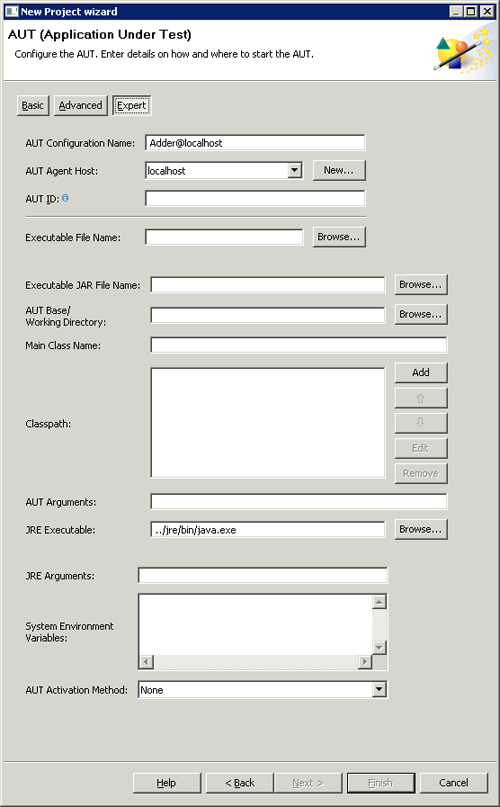
\includegraphics{Tasks/AUTs/PS/autconfigwindow_expert}
\caption{\gdaut configuration window: expert}
\label{autconfigexpert}
\end{center}
\end{figure}

\begin{enumerate}
\item Add any additional desired \bxname{JRE Arguments}. 
\item Enter any required \bxname{System Environment Variables}, in the
format \bxcaption{<VARNAME>=<value>}, i.e. \bxcaption{PATH=C:$\backslash$}. 
Separate each variable with a new line by pressing \bxkey{Enter}.

\bxwarn{Please be advised that ''embedding'' the contents of one
variable into another is not supported at this time by \jb{}. That is,
if you have a variable named \texttt{FOO} whose value is
\bxcaption{abc}, and set the value of a second
variable \texttt{BAR} to \bxcaption{\%FOO\%def}, the second variable will
\emph{not} contain \bxcaption{abcdef}, but rather the exact text
\bxcaption{\%FOO\%def}, without evaluating it.}


\item Select an activation method for your \gdaut{}. 

Activation makes sure that the  \gdaut{} is in focus at the beginning of test execution. This is acheived by clicking somewhere in the \gdaut{} window. You can specify the activation method (i.e. where to click) as part of a configuration for an \gdaut{}, or you can create a \gdstep{} within a test to do the same thing \bxextref{\jb{}efman}{ref,activate}. 

The advantage of specifying an activation method here is that it is central and affects each test execution started on this \gdaut{} with this configuration. 

Bear in mind that you may need to activate your \gdaut{} in order for tests to work, especially if the \gdaut{} runs on the same machine as \jb{}. 


\item Select \bxcaption{Finish} to create this \gdproject{}. 

\end{enumerate}


\clearpage
